\clearpage
\title{Problem 6.2}
\author{}
\date{}
\maketitle

\section*{Problem Description}
Write a program that lets the user type some text, consisting of words separated by blanks, ending with a carriage return, and displays  the text in same word order as entered, "this is a test" becomes "siht si a tset".

\section*{Process}
\subsection*{Code:}

\begin{multicols}{2}{|}
    \begin{minted}[linenos,breaklines,breakanywhere]{nasm}
DATA SEGMENT
    COUNT DW 0
DATA ENDS

CODE SEGMENT
    ASSUME CS:CODE, DS:DATA

START:
    MOV AX, DATA
    MOV DS, AX
    
    XOR CX,CX
    
    MOV AH, 1
    INT 21H

INPUT:
    CMP AL, 0DH
    JE END_
    
    PUSH AX
    INC CX
    INT 21H
    JMP INPUT

END_:
    MOV DX, 0DH
    MOV AH, 2
    INT 21H
    MOV DX, 0AH
    INT 21H
    
    MOV BX, SP
    SUB BX, CX
    SUB BX, CX
    
    XCHG BX, SP
    PUSH 20H
    XCHG BX, SP
    INC COUNT
        
TO_NEW_STK:
    POP DX
    XCHG BX, SP
    PUSH DX
    XCHG BX, SP
    INC COUNT       
    
    LOOP TO_NEW_STK

    MOV CX, COUNT
    MOV COUNT, 0
    PUSH 20H
    INC COUNT 

REVERSE:
    XCHG BX, SP
    POP DX 
    
    XCHG BX, SP
    CMP DL, 20H
    
    JNE SKIP
    
    MOV AH, 2

REV_PRINT:
    POP DX
    INT 21H
    
    DEC COUNT
    JNZ REV_PRINT
    
    MOV DX, 20H

SKIP:
    PUSH DX
    INC COUNT
    
    LOOP REVERSE
    
    MOV AH, 4CH
    INT 21H

CODE ENDS
END START
\end{minted}
\end{multicols}

\subsection*{Output}
\begin{center}
    \centering
    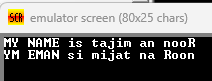
\includegraphics[width = .4\textwidth]{sentRev.png}
    \captionof{figure}{Hexadecimal input \& output}
\end{center}


